\documentclass[a4paper,11pt]{article}
\usepackage[utf8]{inputenc}
\usepackage[english,greek]{babel}
\usepackage{alphabeta}
\usepackage[T1]{fontenc}
\RequirePackage[left=2.00cm, right=2.00cm, top=2.00cm, bottom=2.00cm]{geometry}
\usepackage{nimbusserif,multicol,longtable,multirow,hhline,enumitem,tikz,pgfplots,tkz-euclide,tkz-tab,capt-of,fontawesome5,gensymb}
\let\myBbbk\Bbbk
\let\Bbbk\relax
\usepackage{mtpro2}
\usepackage{xcolor}
\usepackage[explicit]{titlesec}
\usepackage{soul}
\newcommand{\eng}{\selectlanguage{english}}
\newcommand{\gr}{\selectlanguage{greek}}
\newcommand{\hm}[1]{\textrm{ημ}#1}
\newcommand{\syn}[1]{\textrm{συν}#1}
\newcommand{\ef}[1]{\textrm{εφ}#1}
\newcommand{\syf}[1]{\textrm{σφ}#1}

\newcommand{\ekthetesdeiktes}{\DeclareMathSizes{10.95}{10.95}{7}{5}
\DeclareMathSizes{6}{6}{3.8}{2.7}
\DeclareMathSizes{8}{8}{5.1}{3.6}
\DeclareMathSizes{9}{9}{5.8}{4.1}
\DeclareMathSizes{10}{10}{6.4}{4.5}
\DeclareMathSizes{12}{12}{7.7}{5.5}
\DeclareMathSizes{14.4}{14.4}{9.2}{6.5}
\DeclareMathSizes{17.28}{17.28}{11}{7.9}
\DeclareMathSizes{20.74}{20.74}{13.3}{9.4}
\DeclareMathSizes{24.88}{24.88}{16}{11.3}


\makeatletter
\newcommand{\subsup}{
\AtBeginDocument{
\check@mathfonts
\fontdimen16\textfont2=2.5pt
\fontdimen17\textfont2=2.5pt
\fontdimen14\textfont2=4.5pt
\fontdimen13\textfont2=4.5pt}
}
\makeatother}
\usepackage{wrapfig}
\newenvironment{WrapText1}[3][r]
{\wrapfigure[#2]{#1}{#3}}
{\endwrapfigure}

\newenvironment{WrapText2}[3][l]
{\wrapfigure[#2]{#1}{#3}}
{\endwrapfigure}
\newcommand{\wrapr}[6]{
\begin{minipage}{\linewidth}\mbox{}\\
\vspace{#1}
\begin{WrapText1}{#2}{#3}
\vspace{#4}#5\end{WrapText1}#6
\end{minipage}}

\newcommand{\wrapl}[6]{
\begin{minipage}{\linewidth}\mbox{}\\
\vspace{#1}
\begin{WrapText2}{#2}{#3}
\vspace{#4}#5\end{WrapText2}#6
\end{minipage}}
\usepackage{etoolbox,hhline,moreenum}
\usepackage{caption} 
\captionsetup[table]{skip=5pt}
\makeatletter
\newif\ifLT@nocaption
\preto\longtable{\LT@nocaptiontrue}
\appto\endlongtable{%
\ifLT@nocaption
\addtocounter{table}{\m@ne}%
\fi}
\preto\LT@caption{%
\noalign{\global\LT@nocaptionfalse}}
\makeatother

\newlist{alist}{enumerate}{1}
\setlist[alist]{label=\let\textdexiakeraia\relax\alph*.}

\pgfmathdeclarefunction{gauss}{2}{%
  \pgfmathparse{1/(#2*sqrt(2*pi))*exp(-((x-#1)^2)/(2*#2^2))}%
}
\pgfkeys{/pgfplots/aks_on/.style={axis lines=center,
xlabel style={at={(current axis.right of origin)},xshift=1.5ex,anchor=center},
ylabel style={at={(current axis.above origin)},yshift=1.5ex, anchor=center}}}
\pgfkeys{/pgfplots/grafikh parastash/.style={red,line width=.4mm,samples=200}}
\pgfkeys{/pgfplots/belh ar/.style={tick label style={font=\scriptsize},axis line style={-latex}}}
\tikzstyle{pl}=[line width=0.3mm]
\tikzstyle{plm}=[line width=0.4mm]

\newcommand{\kerkissans}[1]{{\fontfamily{maksf}\selectfont {#1}}}
\AtBeginDocument{\renewcommand{\textstigma}{\textsigma\texttau}}

\definecolor{titlecolor}{HTML}{cd0f00}

\newbox\TitleUnderlineTestBox
\newcommand*\TitleUnderline[1]
  {%
    \bgroup
    \setbox\TitleUnderlineTestBox\hbox{\colorbox{titleblue}\strut}%
    \setul{\dimexpr\dp\TitleUnderlineTestBox-.3ex\relax}{.3ex}%
    \ul{#1}%
    \egroup
  }
\newcommand*\SectionNumberBox[1]
  {%
    \colorbox{red!80!black}
      {%
        \makebox[2em][c]
          {%
            \color{white}%
            \strut
            \csname the#1\endcsname
          }%
      }%
    \TitleUnderline{\ \ \ }%
  }
\titleformat{\section}[hang]
    {\Large\bfseries\fontfamily{maksf}\selectfont}%
    {\colorbox{red!80!black}{%
      \raisebox{0pt}[13pt][3pt]{\makebox[80pt]{% height, width
          \color{white}{\kerkissans{\thesection ο Κεφάλαιο}}}%
      }}}%
    {0pt}%
    {\colorbox{black}{\raisebox{0pt}[13pt][3pt]{\color{white}\ #1\ }}}

\titleformat{\subsection}[hang]
    {\large\bfseries\fontfamily{maksf}\selectfont}%
    {\colorbox{red!80!black}{%
      \raisebox{0pt}[13pt][3pt]{\makebox[30pt]{% height, width
          \color{white}{\kerkissans{\thesubsection}}}%
      }}}%
    {0pt}%
    {\colorbox{black}{\raisebox{0pt}[13pt][3pt]{\color{white}\ #1\ }}}

\makeatletter
\@addtoreset{section}{part}
\makeatother

\titleformat{\part}[display]
  {\normalfont\huge\filcenter\bfseries}{}{-30pt}{\Huge \textcolor{red!80!black}{ \kerkissans{ #1}}}
\titlespacing*{\part} 
  {0pt}{0pt}{0pt}

\setlist[enumerate]{itemsep=0mm,label=\thesection.\arabic*}
\definecolor{bblue}{HTML}{4F81BD}
\definecolor{rred}{HTML}{C0504D}
\definecolor{ggreen}{HTML}{9BBB59}
\definecolor{ppurple}{HTML}{9F4C7C}

\makeatletter
\usetikzlibrary{patterns}
\tikzstyle{chart}=[
legend label/.style={font={\scriptsize},anchor=west,align=left},
legend box/.style={rectangle, draw, minimum size=5pt},
axis/.style={black,semithick,->},
axis label/.style={anchor=east,font={\tiny}},
]

\tikzstyle{bar chart}=[
chart,
bar width/.code={
\pgfmathparse{##1/2}
\global\let\bar@w\pgfmathresult
},
bar/.style={very thick, draw=white},
bar label/.style={font={\bf\small},anchor=north},
bar value/.style={font={\footnotesize}},
bar width=.75,
]

\tikzstyle{pie chart}=[
chart,
slice/.style={line cap=round, line join=round,thick,draw=white},
pie title/.style={font={\bf}},
slice type/.style 2 args={
##1/.style={fill=##2},
values of ##1/.style={}
}
]

\pgfdeclarelayer{background}
\pgfdeclarelayer{foreground}
\pgfsetlayers{background,main,foreground}


\newcommand{\pie}[3][]{
\begin{scope}[#1]
\pgfmathsetmacro{\curA}{90}
\pgfmathsetmacro{\r}{1}
\def\c{(0,0)}
\node[pie title] at (90:1.3) {#2};
\foreach \v/\s/\l in{#3}{
\pgfmathsetmacro{\deltaA}{\v/100*360}
\pgfmathsetmacro{\nextA}{\curA + \deltaA}
\pgfmathsetmacro{\midA}{(\curA+\nextA)/2}

\path[slice,\s] \c
-- +(\curA:\r)
arc (\curA:\nextA:\r)
-- cycle;
\pgfmathsetmacro{\d}{max((\deltaA * -(.5/50) + 1) , .5)}

\begin{pgfonlayer}{foreground}
\path \c -- node[pos=\d,pie values,values of \s]{$\l$} +(\midA:\r);
\end{pgfonlayer}

\global\let\curA\nextA
}
\end{scope}
}

\newcommand{\legend}[2][]{
\begin{scope}[#1]
\path
\foreach \n/\s in {#2}
{
++(0,-10pt) node[\s,legend box] {} +(5pt,0) node[legend label] {\n}
}
;
\end{scope}
}
\definecolor{a}{cmyk}{0,1,1,0.05}
\definecolor{b}{cmyk}{0,.8,.8,.15}
\definecolor{c}{cmyk}{0,.8,.8,.0}
\definecolor{d}{cmyk}{0,.7,.7,0}
\definecolor{e}{cmyk}{0,.5,.5,0}


\pgfplotsset{every axis/.append style={
x tick label style={/pgf/number format/.cd, 1000 sep={.}}}}


\begin{document}
\begin{center}
\includegraphics[width=0.4\linewidth]{/home/spyros/texmf/tex/latex/local/frontisthrio/Logotypo-Filomatheia_1}\\
\vspace{-1mm}
{\faIcon{map-marker-alt}} : Ιακώβου Πολυλά 24 - \ Πεζόδρομος\,\,|\,\,{\faIcon{phone-alt}} : 26610 20144\,\,|\,\, {\faIcon{mobile-alt}} : 6932327283 - 6955058444\\
\rule{14.7cm}{.1mm}\\
\vspace{2mm}
{\bf\today}\\
\vspace*{4cm}
{\huge \textbf{ΤΥΠΟΛΟΓΙΟ ΚΑΙ ΜΕΘΟΔΟΛΟΓΙΑ}\\[3mm]\textbf{ΒΑΣΙΚΩΝ ΑΣΚΗΣΕΩΝ}}
\vspace*{\fill}
\vfil
Φρόνιμος Σπύρος
\end{center}
\pagenumbering{gobble}
\newpage
\null
\newpage
\pagenumbering{arabic}
\begin{center}
\part{Τυπολόγιο}
\end{center}
\section{Διαφορικός Λογισμός}
\subsection{Συναρτήσεις}
\begin{enumerate}[label=\thesection.\arabic*]
\item Πεδίο ορισμού συνάρτησης $D_f$
\end{enumerate}
\begin{center}
\begin{tabular}{ccc}
\hline 
\rule[-2ex]{0pt}{5ex} \textbf{Είδος} & \textbf{Τύπος} & \textbf{Περιορισμός} \\ \hhline{===} 
\rule[-2ex]{0pt}{5ex} Πολυωνυμική & 
 $ f(x)=A(x) $ & $ - $ \\
\rule[-2ex]{0pt}{5ex} Ρητή & 
 $ f(x)=\dfrac{A(x)}{B(x)} $ & $ B(x)\neq 0 $ \\ \rule[-2ex]{0pt}{5ex} Άρρητη & 
 $ f(x)=\sqrt{A(x)} $ & $ A(x)\geq 0 $ \\
\rule[-2ex]{0pt}{5ex} Άρρητος παρονομαστής & 
$ f(x)=\dfrac{A(x)}{\sqrt{B(x)}} $ & $ B(x)>0 $ \\
\rule[-2ex]{0pt}{5ex} Ημίτονο - Συνημίτονο & 
$ f(x)=\hm{A(x)} $ ή $f(x)=\syn{A(x)}$ & $ - $ \\
\rule[-2ex]{0pt}{5ex} Εφαπτομένη & 
$ f(x)=\ef{A(x)} $ & $ A(x)\neq \kappa\pi+\frac{\pi}{2} $ \\
\rule[-2ex]{0pt}{5ex} Συνεφαπτομένη & 
$ f(x)=\syf{A(x)} $ & $ A(x)\neq\kappa\pi $ \\
\hline 
\end{tabular}\captionof{table}{Πεδίο ορισμού βασικών συναρτήσεων}\label{pinakas}
\end{center}
\begin{enumerate}[resume]
\item Πράξεις συναρτήσεων
\begin{itemize}
\item Άθροισμα : $(f+g)(x)=f(x)+g(x)\ \ ,\ \ D_{f+g}=D_f\cap D_g$
\item Διαφορά : $(f-g)(x)=f(x)-g(x)\ \ ,\ \ D_{f-g}=D_f\cap D_g$
\item Γινόμενο : $(f\cdot g)(x)=f(x)\cdot g(x)\ \ ,\ \ D_{f\cdot g}=D_f\cap D_g$
\item Πηλίκο : $\left(\frac{f}{g}\right)(x)=\frac{f(x)}{g(x)}\ \ ,\ \ D_{f/g}=D_f\cap D_g-\{x|g(x)=0\}$
\end{itemize}
\item Το σημείο $ M(a,\beta) $ ανήκει στη $C_f\Leftrightarrow f(a)=\beta$.
\item Σημείο τομής της $C_f$ μέ τον άξονα
\begin{multicols}{2}
\begin{itemize}
\item $x'x : f(x)=0$
\item $y'y : A(0,f(0))$
\end{itemize}
\end{multicols}
\item Σχετική θέση $C_f$ με τον άξονα $x'x$
\begin{itemize}
\item Η $C_f$ είναι πάνω από τον $x'x\Rightarrow f(x)>0$
\item Η $C_f$ είναι κάτω από τον $x'x\Rightarrow f(x)<0$
\end{itemize}
\item Σχετική θέση $C_f$ με $C_g$
\begin{itemize}
\item Η $C_f$ είναι πάνω από την $C_g\Rightarrow f(x)>g(x)$
\item Η $C_f$ είναι κάτω από την $C_g\Rightarrow f(x)<g(x)$
\end{itemize}
\item Γνησίως αύξουσα συνάρτηση $f\uparrow\varDelta $
\[x_1<x_2\Rightarrow f(x_1)<f(x_2)\] 
Γνησίως φθίνουσα συνάρτηση $f\downarrow\varDelta$
\[x_1<x_2\Rightarrow f(x_1)<f(x_2)\] 
\item Ακρότατα της $f$
\begin{itemize}
\item Ολικό μέγιστο στη θέση $x_0$ : $f(x)\leq f(x_0)$ για κάθε $x\in D_f $
\item Ολικό ελάχιστο στη θέση $ x_0 $ : $f(x)\geq f(x_0)$ για κάθε $x\in D_f$.
\item Τοπικό μέγιστο στη θέση $x_0$ : $f(x)\leq f(x_0)$ για κάθε $x$ σε μία περιοχή του $x_0$.
\item Ολικό ελάχιστο στη θέση $ x_0 $ : $f(x)\geq f(x_0)$ για κάθε $x$ σε μία περιοχή του $x_0$.
\end{itemize}
\end{enumerate}
\subsection{Όρια - Συνέχεια}
\begin{enumerate}[resume]
\begin{multicols}{2}
\item Όριο συνάρτησης στο $x_0$ : $\lim\limits_{x\to x_0}{f(x)}$
\item Συνέχεια σε σημείο $x_0$: $\lim\limits_{x\to x_0}{f(x)}=f(x_0)$
\end{multicols}
\item Ιδιότητες ορίων : 
\end{enumerate}
\begin{center}
\begin{tabular}{cc}
\hline
\rule[-2ex]{0pt}{5ex} \textbf{Πράξη} & \textbf{Ιδιότητα} \\
\hhline{==}
\rule[-2ex]{0pt}{5ex} Άθροισμα & $\lim\limits_{x\to x_0}(f(x)+g(x))=\lim\limits_{x\to x_0}f(x)+\lim\limits_{x\to x_0}g(x)$  \\
\rule[-2ex]{0pt}{5ex} Πολλαπλάσιο & $\lim\limits_{x\to x_0}(\kappa f(x))=\kappa\lim\limits_{x\to x_0}f(x)$ \\
\rule[-2ex]{0pt}{5ex} Γινόμενο & $\lim\limits_{x\to x_0}(f(x)\cdot g(x))=\lim\limits_{x\to x_0}f(x)\cdot\lim\limits_{x\to x_0}g(x)$ \\
\rule[-2ex]{0pt}{7ex} Πηλίκο & $\lim\limits_{x\to x_0}\frac{f(x)}{g(x)}=\dfrac{\lim\limits_{x\to x_0}f(x)}{\lim\limits_{x\to x_0}g(x)}$ \\
\rule[-2ex]{0pt}{6ex} Δύναμη & $\lim\limits_{x\to x_0}(f(x))^{\nu}=\left(\lim\limits_{x\to x_0}f(x)\right)^{\nu}$ \\[4mm]
\rule[-2ex]{0pt}{5ex} Ρίζα & $\lim\limits_{x\to x_0}\sqrt[\nu]{f(x)}=\sqrt[\nu]{\lim\limits_{x\to x_0}f(x)}$ \\
\hline
\end{tabular}\captionof{table}{Ιδιότητες των ορίων}
\end{center}
\subsection{Παράγωγος}
\begin{enumerate}[resume]
\item Παράγωγος σε σημείο $x_0$ : $f'(x_0)=\lim\limits_{h\to 0}{\dfrac{f(x_0+h)-f(x_0)}{h}}$
\item Παράγωγος συνάρτηση : $f'(x)=\lim\limits_{h\to 0}{\dfrac{f(x+h)-f(x)}{h}}$
\end{enumerate}
\begin{center}
\textbf{ΠΙΝΑΚΑΣ ΠΑΡΑΓΩΓΩΝ ΒΑΣΙΚΩΝ ΣΥΝΑΡΤΗΣΕΩΝ}
\begin{longtable}{cc|ccc}
\hline  \multicolumn{2}{c|}{\textbf{ΑΠΛΕΣ}} & \multicolumn{3}{c}{\textbf{ΣΥΝΘΕΤΕΣ}} \rule[-2ex]{0pt}{5.5ex} \\ 
\hline \rule[-2ex]{0pt}{5.5ex} Συνάρτηση $ f $& Παράγωγος $ f' $ & Συνάρτηση $ g\circ f $ & Παράγωγος $ \left( g\circ f \right)' $ & Περιγραφή\\ 
\hhline{=====} \rule[-2ex]{0pt}{5.5ex} $ c $ & $ 0 $ &  &  & \\ 
\rule[-2ex]{0pt}{5ex} $ x $ & $ 1 $ &  &  &  \\ 
\rule[-2ex]{0pt}{5ex} $ x^\nu $ & $ \nu x^{\nu-1} $ & $ f^\nu(x) $ & $ \nu f^{\nu-1}(x)\cdot f'(x) $ & $ \nu(\text{βάση})^{\nu-1}(\text{βάση})' $ \\ 
\rule[-2ex]{0pt}{5ex} $ \dfrac{1}{x} $ & $ -\dfrac{1}{x^2} $ & $ \dfrac{1}{f(x)} $ & $ -\dfrac{f'(x)}{f^2(x)} $ &$ -\dfrac{(\text{Παρονομαστής})'}{\text{Παρονομαστής}^2} $ \\ 
\rule[-2ex]{0pt}{7ex} $ \sqrt{x} $ & $ \dfrac{1}{2\!\sqrt{x}} $ & $ \sqrt{f(x)} $ & $ \dfrac{f'(x)}{2\!\sqrt{f(x)}} $ & $ \dfrac{(\text{Υπόριζο})'}{2\cdot\text{Ρίζα}} $ \\ 
\rule[-2ex]{0pt}{5ex} $ \hm{x} $ & $ \syn{x} $ & $ \hm{f(x)} $ & $ \syn{f(x)}\cdot f'(x) $ & $ \syn{(\text{Γωνία})\cdot(\text{Γωνία})'} $ \\ 
\rule[-2ex]{0pt}{5ex} $ \syn{x} $ & $ -\hm{x} $ & $ \syn{f(x)} $ & $ -\hm{f(x)}\cdot f'(x) $ &$ -\hm{(\text{Γωνία})\cdot(\text{Γωνία})'} $\\ 
\rule[-2ex]{0pt}{5ex} $ \ef{x} $ & $ \dfrac{1}{\syn^2{x}} $ & $ \ef{f(x)} $ & $ \dfrac{f'(x)}{\syn^2{f(x)}} $ & $ \dfrac{(\text{Γωνία})'}{\syn^2{(\text{Γωνία})}} $ \\ 
\rule[-2ex]{0pt}{7ex} $ \syf{x} $ & $ -\dfrac{1}{\hm^2{x}} $ & $ \syf{f(x)} $ & $ -\dfrac{f'(x)}{\hm^2{f(x)}} $ & $ -\dfrac{(\text{Γωνία})'}{\hm^2{(\text{Γωνία})}} $ \\ 
\hline 
\end{longtable}\captionof{table}{Παράγωγοι απλών και σύνθετων συναρτήσεων}\label{pinakas1}
\end{center}
\begin{center}
\vspace{5mm}
\textbf{ΚΑΝΟΝΕΣ ΠΑΡΑΓΩΓΙΣΗΣ}\\
\vspace{5mm}
\begin{tabular}{ccc}
\hline 
\rule[-2ex]{0pt}{5ex} \textbf{Πράξη} & \textbf{Συνάρτηση} & \textbf{Παράγωγος} \\ 
\hhline{===}
\rule[-2ex]{0pt}{5ex} \textbf{Άθροισμα - Διαφορά} & $ f(x)\pm g(x) $ & $ f'(x)\pm g'(x) $ \\ 
\rule[-2ex]{0pt}{5ex} \textbf{Πολλαπλάσιο} & $ c\cdot f(x) $ & $ c\cdot f'(x) $ \\  
\rule[-2ex]{0pt}{5ex} \textbf{Γινόμενο} & $ f(x)\cdot g(x) $ & $ f'(x)\cdot g(x)+f(x)\cdot g'(x) $ \\ 
\rule[-2ex]{0pt}{5ex} \textbf{Πηλίκο} & $ \dfrac{f(x)}{g(x)} $ & $ \dfrac{f'(x)\cdot g(x)-f(x)\cdot g'(x)}{g^2(x)} $ \\  
\rule[-2ex]{0pt}{5ex} \textbf{Σύνθεση} & $ f(g(x)) $ & $ f'(g(x))\cdot g'(x) $ \\ 
\hline 
\end{tabular}\captionof{table}{Κανόνες παραγώγισης πράξεων}\label{pinakas2}
\end{center}
\subsection{Εφαπτομένη - Ρυθμός μεταβολής}
\begin{enumerate}[resume]
\item Εξίσωση εφαπτομένης σε σημείο $M(x_0,f(x_0))$ : $y=\lambda x+\beta$ 
\item Συντελεστής διεύθυνσης εφαπτομένης : $\lambda=f'(x_0)=\textrm{εφ}{\omega}$
\item Ρυθμός μεταβολής μιας συνάρτησης $f$ σε σημείο $x_0$ : $f'(x_0)$
\end{enumerate}
\section{Στατιστική}
\subsection{Βασικές έννοιες - Πίνακες συχνοτήτων}
\begin{enumerate}[label=\thesection.\arabic*]
\begin{multicols}{2}
\item $\nu : $ μέγεθος δείγματος
\item $\kappa : $Πλήθος τιμών μεταβλητής $X$
\item $t_1,t_2,\ldots,t_{\nu} : $ Παρατηρήσεις του δείγματος
\item $x_1,x_2,\ldots,x_{\kappa} : $ Τιμές μεταβλητής $X$.
\item $\nu_i,i=1,\ldots,\kappa : $ Συχνότητα της τιμής $x_i$.
\item $f_i,i=1,\ldots,\kappa : $ Σχετική συχνότητα της τιμής $x_i$.
\item $f_i\%,i=1,\ldots,\kappa : $ Σχετική συχνότητα επί τοις $100$ της τιμής $x_i$.
\end{multicols}
\item Ιδιότητες που αφορούν τη συχνότητα $ \nu_i $
\begin{alist}
\item $ 0\leq\nu_i\leq\nu $ για $i=1,2,\ldots,\kappa$.
\item $ \nu_1+\nu_2+\ldots+\nu_\kappa=\nu $
\item $ \nu_i=N_i-N_{i-1} $ για $i=1,2,\ldots,\kappa$.
\end{alist}
\item Ιδιότητες που αφορούν τη συχνότητα $f_i$
\begin{alist}
\item $f_i=\dfrac{\nu_i}{\nu}$ και $f_i\%=\dfrac{\nu_i}{\nu}\cdot 100$  για $i=1,2,\ldots,\kappa$.
\item $ 0\leq f_i\leq 1\ \textrm{ και }\ 0\leq f_i\%\leq100 $  για $i=1,2,\ldots,\kappa$.
\item $ f_1+f_2+\ldots+f_\kappa=1\ \textrm{ και }\ f_1\%+f_2\%+\ldots+f_\kappa\%=100 $
\item $ f_i=F_i-F_{i-1} $ για $i=1,2,\ldots,\kappa$.
\item $ f_i\%=F_i\%-F_{i-1}\% $ για $i=1,2,\ldots,\kappa$.
\end{alist}
\item Ιδιότητες που αφορούν την αθροιστική συχνότητα $N_i$
\begin{alist}
\item $ N_i=\nu_1+\nu_2+\ldots+\nu_i $ για $i=1,2,\ldots,\kappa$.
\begin{multicols}{3}
\item $N_i=N_{i-1}+\nu_i$
\item $ N_1=\nu_1 $
\item $ N_\kappa=\nu $ για $i=1,2,\ldots,\kappa$.
\end{multicols}
\end{alist}
\item Ιδιότητες που αφορούν την αθροιστική σχετική συχνότητα $F_i$
\begin{alist}
\item $ F_i=f_1+f_2+\ldots+f_i$  για $i=1,2,\ldots,\kappa$.
\item $ F_i=\frac{N_i}{\nu} $ για $i=1,2,\ldots,\kappa$.
\item $ F_i\%=f_1\%+f_2\%+\ldots+f_i\% $ για $i=1,2,\ldots,\kappa$.
\item $ F_i\%=\frac{N_i}{\nu}\cdot 100 $ για $i=1,2,\ldots,\kappa$.
\begin{multicols}{2}
\item $ F_1=f_1 $
\item $ F_1\%=f_1\% $
\item $ F_\kappa=1 $
\item $ F_\kappa\%=100 $
\end{multicols}
\end{alist}
\end{enumerate}
\subsection{Παρουσίαση στατιστικών δεδομένων - Σχήματα}
\begin{enumerate}[resume]
\item Μέτρο τόξου της τιμής $x_i$ σε κυκλικό διάγραμμα : $a_i=\dfrac{\nu_i}{\nu}\cdot 360\degree=f_i\cdot 360\degree$.
\end{enumerate}
\begin{center}
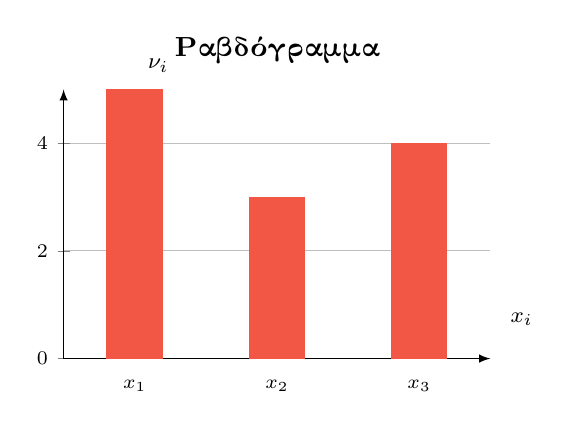
\begin{tikzpicture}
\begin{axis}[axis lines=left,belh ar,
width  = 7cm,
height = 5cm,
major x tick style = transparent,
ybar=2*\pgflinewidth,
bar width=20pt,ylabel={\footnotesize \rotatebox{-90}{$ \nu_i $}},xlabel={\footnotesize $ x_i $},xlabel style={at={(current axis.right of origin)},xshift=4mm,yshift=5mm, anchor=center},ylabel style={at={(current axis.above origin)},xshift=3mm,yshift=-3mm,,anchor=center},
ymajorgrids = true,
symbolic x coords={$ x_1 $,$ x_2 $,$ x_3 $},
xtick = data,
scaled y ticks = false,
enlarge x limits=0.25,
ymin=0,title={\textbf{Ραβδόγραμμα}},
legend cell align=left,
legend style={at={(1,1.05)},anchor=south east,
column sep=1ex}]
\addplot[style={d,fill=d,mark=none}]
coordinates {($ x_1 $, 5.0) ($ x_2 $,3.0) ($ x_3 $,4.0)};
%\legend{Μαθηματικά,Φυσική,TreeScore $>3$,TreeScore $>4$}
\end{axis}
\end{tikzpicture}\quad
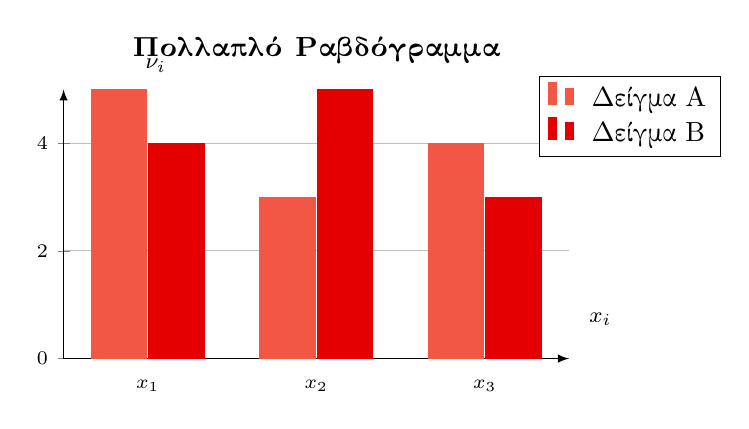
\begin{tikzpicture}
\begin{axis}[axis lines=left,belh ar,
width  = 8cm,
height = 5cm,
major x tick style = transparent,title={\textbf{Πολλαπλό Ραβδόγραμμα}},
ybar=2*\pgflinewidth,
bar width=20pt,ylabel={\footnotesize \rotatebox{-90}{$ \nu_i $}},xlabel={\footnotesize $ x_i $},xlabel style={at={(current axis.right of origin)},xshift=4mm,yshift=5mm, anchor=center},ylabel style={at={(current axis.above origin)},xshift=3mm,yshift=-1mm,,anchor=center},
ymajorgrids = true,
symbolic x coords={$ x_1 $,$ x_2 $,$ x_3 $},
xtick = data,
scaled y ticks = false,
enlarge x limits=0.25,
ymin=0,
legend cell align=left,
legend style={at={(1.3,1.05)},anchor=north east,
column sep=1ex}]
\addplot[style={d,fill=d,mark=none}]
coordinates {($ x_1 $, 5.0) ($ x_2 $,3.0) ($ x_3 $,4.0)};
\addplot[style={red!90!black,fill=red!90!black,mark=none}]
coordinates {($ x_1 $, 4.0) ($ x_2 $,5.0) ($ x_3 $,3.0)};
\legend{Δείγμα Α,Δείγμα Β}
\end{axis}
\end{tikzpicture}\\
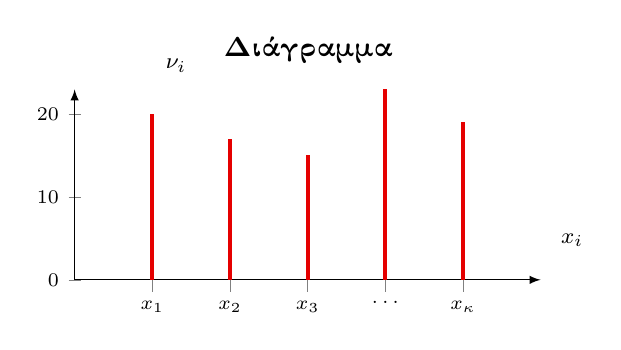
\begin{tikzpicture}
\begin{axis}[axis lines=left,belh ar,ybar,enlarge x limits=0.25,bar width=1pt,ymin=0,ylabel={\footnotesize \rotatebox{-90}{$ \nu_i $}},xlabel={\footnotesize $ x_i $},xlabel style={at={(current axis.right of origin)},xshift=4mm,yshift=5mm, anchor=center},ylabel style={at={(current axis.above origin)},xshift=3mm,yshift=-3mm,,anchor=center},height=4cm,width=7.5cm,symbolic x coords={$ x_1 $,$ x_2 $,$ x_3 $,$\ldots$,$ x_\kappa $},
xtick = data,title={\textbf{Διάγραμμα}}]
\addplot
[draw=red!90!black,fill=red!90!black] 
coordinates
{($ x_1 $,20) ($ x_2 $,17) ($ x_3 $,15) ($\ldots$,23) ($ x_\kappa $,19)};
\end{axis}
\end{tikzpicture}\quad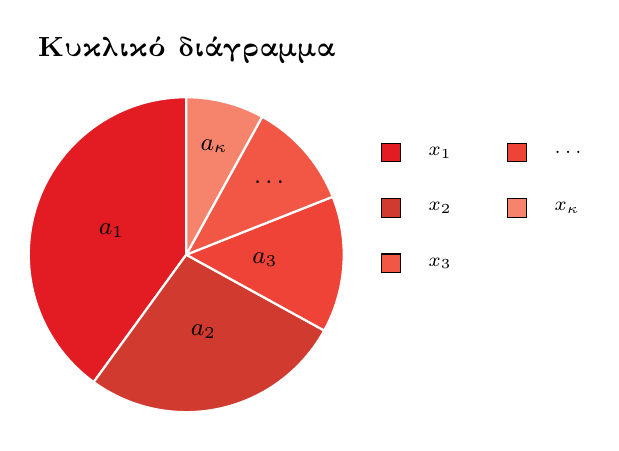
\begin{tikzpicture}
[pie chart,slice type={comet}{a},
slice type={legno}{b},
slice type={coltello}{d},
slice type={sedia}{c},
slice type={caffe}{e},
pie values/.style={font={\small}},
scale=2
]
\node at (0,1.3) {\textbf{Κυκλικό διάγραμμα}};
\pie[values of coltello/.style={pos=.7}]{}{40/comet/a_1,27/legno/a_2,14/sedia/a_3,11/coltello/\ldots,8/caffe/a_\kappa}


\legend[shift={(1.3cm,1cm)}]{{$ x_1 $}/comet, {$ x_2 $}/legno, {$ x_3 $}/coltello}
\legend[shift={(2.1cm,1cm)}]{{$ \ldots $}/sedia, {$ x_\kappa $}/caffe}

\end{tikzpicture}
\end{center}
\subsection{Ομαδοποιημένες παρατηρήσεις}
\wrapr{-15mm}{5}{7.1cm}{-2mm}{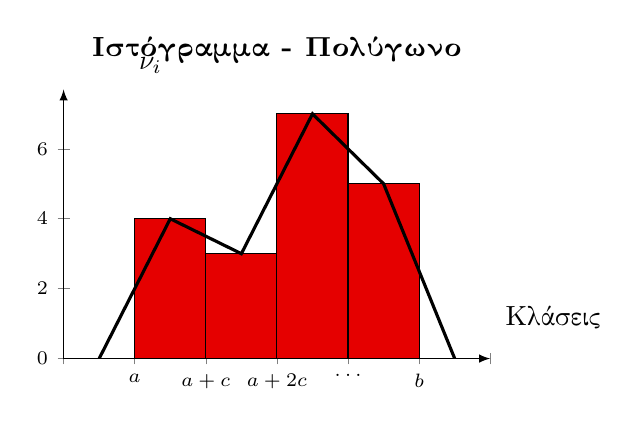
\begin{tikzpicture}
\begin{axis}[axis lines=left,belh ar,width=7cm,
height=5cm,xmin=-2,xmax=10,xlabel style={at={(current axis.right of origin)},xshift=8mm,yshift=5mm, anchor=center},
ylabel style={at={(current axis.above origin)},yshift=-2mm,xshift=3mm,anchor=center},
ymin=0, ymax=7.7,xlabel={Κλάσεις},ylabel={\rotatebox{-90}{$ \nu_i $}},xticklabels={,,$a$,$a+c$,$a+2c$,$\ldots$,$b$},title={\textbf{Ιστόγραμμα - Πολύγωνο}}]
\draw[fill=red!90!black] (axis cs:0,0) rectangle (axis cs:2,4);
\draw[fill=red!90!black] (axis cs:2,0) rectangle (axis cs:4,3);
\draw[fill=red!90!black] (axis cs:4,0) rectangle (axis cs:6,7);
\draw[fill=red!90!black] (axis cs:6,0) rectangle (axis cs:8,5);
\draw[plm] (axis cs:-1,0)--(axis cs:1,4)--(axis cs:3,3)--(axis cs:5,7)--(axis cs:7,5)--(axis cs:9,0);
\end{axis}
\end{tikzpicture}}{
\begin{enumerate}[resume]
\item Εύρος παρατηρήσεων $ R=t_{\max}-t_{\min} $
\item Πλάτος κλάσης $ c=\dfrac{R}{\kappa} $ όπου $ \kappa $ το πλήθος των κλάσεων.
\item Κεντρική τιμή της κλάσης $ [a,\beta) $
\begin{itemize}
\item $ x_i=\dfrac{a+\beta}{2},i=1,\ldots,\kappa $
\item $x_i=x_{i-1}+c,\ i=2,\ldots,\kappa$
\end{itemize}
\end{enumerate}}

\subsection{Μέτρα θέσης}
\begin{enumerate}[resume]
\item Μέση τιμή :
\begin{alist}
\item Με παρατηρήσεις $t_i : \bar{x}=\dfrac{t_1+t_2+\ldots+t_\nu}{\nu}=\dfrac{1}{\nu}\displaystyle\sum\limits_{i=1}^{\nu}{t_i} $
\item Με συχνότητες $\nu_i$
$ \bar{x}=\dfrac{1}{\nu}\displaystyle\sum\limits_{i=1}^{\kappa}{x_i\nu_i}$
\item Με συχνότητες $ f_i :  \bar{x}=\displaystyle\sum\limits_{i=1}^{\kappa}{x_if_i} $
\end{alist}\label{meshtimh}
\item Σταθμικός μέσος : $\bar{x}=\dfrac{t_iw_1+t_2w_2+\ldots+t_\nu w_\nu}{w_1+w_2+\ldots+w_\nu}=\dfrac{\sum\limits_{i=1}^{\nu}{t_iw_i}}{\sum\limits_{i=1}^{\nu}{w_i}} $
όπου $ w_i\ ,\ i=1,2,\ldots,\nu $ είναι οι συντελεστές βαρύτητας των παρατηρήσεων.\label{stahmikos}
\item Διάμεσος 
\begin{alist}
\begin{multicols}{2}
\item $\delta=t_{\frac{v+1}{2}}$ για $\nu$: περιττό
\item $\delta=\dfrac{t_{\frac{\nu}{2}}+t_{\frac{\nu}{2}+1}}{2}$ για $\nu$: άρτιο
\end{multicols}
\item Διάμεσος σε ομαδοποιημένα δεδομένα
\begin{multicols}{2}
\begin{itemize}
\item 
$\delta=L_i+\dfrac{c}{\nu_i}\left(\dfrac{\nu}{2}-N_{i-1}\right)$.
\item 
$\delta=L_i+\dfrac{c}{f_i\%}\left(50-F_{i-1}\%\right)$.
\end{itemize}
\end{multicols}
όπου $i:$ ο δείκτης της κλάσης στην οποία ξεπερνάμε 1η φορά ή συναντάμε το μισό δείγμα (βλέπε μέθοδο \ref{diamesos1} και \ref{diamesos2})
\end{alist}
\end{enumerate}
\subsection{Μέτρα διασποράς}
\begin{enumerate}[resume]
\item Εύρος : $ R=t_{max}-t_{min} $
\item Διακύμανση\label{diakymansh}
\begin{alist}
\item Για ακέραιο μέσο όρο: $ s^2=\dfrac{1}{\nu}\displaystyle\sum_{i=1}^{\nu}{(t_i-\bar{x})^2} $
\item Για μη ακέραιο μέσο όρο $ s^2=\dfrac{1}{\nu}\LEFTRIGHT\{\}{\sum\limits_{i=1}^{\nu}{t_i^2}-\frac{\left( \sum\limits_{i=1}^{\nu}{t_i}\right)^2 }{\nu}} $
\item Με συχνότητα $\nu_i$ : $ s^2=\dfrac{1}{\nu}\displaystyle\sum\limits_{i=1}^{\kappa}{(x_i-\bar{x})^2\nu_i} $ για ακέραιο μέσο όρο.
\item Με συχνότητα $\nu_i$ : $ s^2=\dfrac{1}{\nu}\LEFTRIGHT\{\}{\sum\limits_{i=1}^{\kappa}{x_i^2\nu_i}-\frac{\left( \sum\limits_{i=1}^{\kappa}{x_i\nu_i}\right)^2 }{\nu}} $ για μη ακέραιο μέσο όρο.
\item Με συχνότητα $f_i$ : $ s^2=\displaystyle\sum\limits_{i=1}^{\kappa}{x_i^2f_i-(\bar{x})^2} $
\end{alist}
\item Σχέση μεταξύ διακύμανσης και μέσης τιμής : $s^2=\overline{x^2}-\bar{x}^2$ όπου $\overline{x^2}=\frac{1}{\nu}\displaystyle\sum\limits_{i=1}^{\infty}{t_i^2}$
\item Τυπική απόκλιση $ s=\sqrt{s^2} $
\item Συντελεστής μεταβλητότητας $ CV=\dfrac{s}{|\overline{x}|}\cdot 100\% $
\begin{itemize}
\item Αν $CV\leq 10\%$ τότε το δείγμα είναι ομοιογενές.
\item Αν $CV_A<CV_B$ τότε το δείγμα $A$ έχει μεγαλύτερη ομοιογένεια από το $B$.
\end{itemize}
\item Κανονική κατανομή
\begin{center}
\begin{tikzpicture}
\begin{axis}[axis y line=none,aks_on,belh ar,
  no markers,xmax=8, samples=200,
  axis lines*=left, xlabel=$x_i$, ylabel=$\nu_i$,
  every axis y label/.style={at=(current axis.above origin),anchor=south},ymin=0,
  every axis x label/.style={at=(current axis.right of origin),anchor=west},
  height=4.5cm, width=12cm,xticklabels={$ \bar{x}-3s $,$ \bar{x}-2s $,$ \bar{x}-s $,$ \bar{x} $,$ \bar{x}+s $,$ \bar{x}+2s $,$ \bar{x}+3s $},  xtick={1,2,3,4,5,6,7},enlargelimits=false, clip=false, axis on top]
\addplot [thick,fill=red!10,domain=0:1] {gauss(4,1)+0.015} \closedcycle;\addplot [fill=red!30, domain=1:2] {gauss(4,1)+0.015} \closedcycle;
\addplot [fill=red!10, domain=2:3] {gauss(4,1)+0.015} \closedcycle;
\addplot [fill=red!30, domain=3:4] {gauss(4,1)+0.015} \closedcycle;
\addplot [fill=red!30, domain=4:5] {gauss(4,1)+0.015} \closedcycle;
\addplot [fill=red!10, domain=5:6] {gauss(4,1)+0.015} \closedcycle;
\addplot [fill=red!30, domain=6:7] {gauss(4,1)+0.015} \closedcycle;
\addplot [fill=red!10, domain=7:8] {gauss(4,1)+0.015} \closedcycle;
\addplot [plm,draw=red!80!black,domain=0:8] {gauss(4,1)+0.015};
\node at (axis cs:3.5,0.15){\footnotesize$34\%$};
\node at (axis cs:4.5,0.15){\footnotesize$34\%$};
\node at (axis cs:5.5,0.05){\footnotesize$13.5\%$};
\node at (axis cs:6.5,0.08){\footnotesize$2.35\%$};
\node at (axis cs:7.5,0.08){\footnotesize$0.15\%$};
\node at (axis cs:2.5,0.05){\footnotesize$13.5\%$};
\node at (axis cs:1.5,0.08){\footnotesize$2.35\%$};
\node at (axis cs:0.5,0.08){\footnotesize$0.15\%$};
\draw[latex-latex] (axis cs:3,-.09)--(axis cs:5,-.09)node[pos=0.5,below] {$68\%$};
\draw[latex-latex] (axis cs:2,-.17)--(axis cs:6,-.17)node[pos=0.5,below] {$95\%$};
\draw[latex-latex] (axis cs:1,-.25)--(axis cs:7,-.25)node[pos=0.5,below] {$99.7\%$};
\end{axis}
\end{tikzpicture}
\end{center}
\item Μεταβολές των παρατηρήσεων\\
Δίνονται οι παρατηρήσεις $x_1,x_2,\ldots,x_\nu$ μιας μεταβλητής $X$, με μέση τιμή $\bar{x}$ και τυπική απόκλιση $s_x$. Οι μεταβολές στις τιμές αυτές  επηρεάζουν τη μέση τιμή και την τυπική απόκλιση σύμφωνα με τον ακόλουθο πίνακα.
\begin{center}
\begin{tabular}{|c|c|c|c|}\hline \rule[-2ex]{0mm}{5.5ex} Αλλαγή &
Τελικές τιμές & Νέα μέση τιμή & Νέα τυπική απόκλιση\\
\hhline{====} \rule[-2ex]{0mm}{5.5ex} Αύξηση - Μείωση & $y_i=x_i\pm c$ & $\bar{y}=\bar{x}\pm c$ & $s_y=s_x$\\
Πολλαπλασιασμός &\rule[-2ex]{0mm}{5.5ex}$y_i=x_i\cdot c$ & $\bar{y}=\bar{x}\cdot c$ & $s_y=s_x\cdot |c|$\\
Διαίρεση &\rule[-2ex]{0mm}{5.5ex}$y_i=\dfrac{x_i}{c}$ & $\bar{y}=\dfrac{\bar{x}}{c}$ & $s_y=\dfrac{s_x}{|c|}$\\
Αύξηση κατά $a\%$ &\rule[-2ex]{0mm}{5.5ex}$y_i=x_i\left(1+a\%\right)$ & $\bar{y}=\bar{x}\left(1+a\%\right)$ & $s_y=s_x\left(1+a\%\right)$\\
Μείωση κατά $a\%$ &\rule[-2ex]{0mm}{5.5ex}$y_i=x_i\left(1-a\%\right)$ & $\bar{y}=\bar{x}\left(1-a\%\right)$ & $s_y=s_x\left(1-a\%\right)$\\
Μέρος &\rule[-2ex]{0mm}{5.5ex}$y_i=x_i\cdot a\%$ & $\bar{y}=\bar{x}\cdot a\%$ & $s_y=s_x\cdot a\%$\\
Συνδυασμός &\rule[-2ex]{0mm}{5.5ex}$y_i=\lambda\cdot x_i\pm c$ & $\bar{y}=\lambda\cdot\bar{x}\pm c$ & $s_y=|\lambda|s_x$\\
\hline
\end{tabular}\captionof{table}{Υπολογισμός νέας μέσης τιμής και τυπικής απόκλισης από μεταβολές παρατηρήσεων}\label{pinakas3}
\end{center}
\end{enumerate}
\newpage
\begin{center}
\part{Βασικά είδη ασκήσεων}
\end{center}
\section{Διαφορικός λογισμός}
\begin{enumerate}[label=\bf\thesection.\arabic*.]
\item\textbf{Συνέχεια συνάρτησης σε σημείο}
\begin{itemize}
\item Υπολογίζουμε το όριο της $ f $ στο σημείο $ x_0 $: $\lim\limits_{x\to x_0}{f(x)}$
\item Υπολογίζουμε την τιμή $f(x_0)$.
\end{itemize}
Αν είναι ίσα τότε η συνάρτηση είναι συνεχής στο $x_0$.
\item\textbf{Όριο της μορφής $\frac{0}{0}$ σε σημείο $ x_0 $}
\begin{itemize}
\item Αν η συνάρτηση είναι ρητή τότε παραγοντοποιούμε τα πολυώνυμα ώσπου να εμφανιστεί η παράσταση $ x-x_0 $ και να απλοποιηθεί.
\item Αν η συνάρτηση περιέχει ρίζα, πολλαπλασιάζουμε πάνω και κάτω με τη συζυγή παράσταση του όρου που έχει τη ρίζα. Στη συνέχεια κάνουμε πράξεις μέχρι να διαιρεθεί η παράσταση $x-x_0$. Τέλος υπολογίζουμε το όριο.
\end{itemize}
\item\textbf{Παράγωγος απλών - σύνθετων συναρτήσεων}\\
Για να υπολογίσουμε τις παραγώγους απλών ή και σύνθετων συναρτήσεων ακολουθούμε τον πίνακα \ref{pinakas1} καθώς και τους κανόνες παραγώγισης πίνακα \ref{pinakas2} για τις πράξεις.
\item\textbf{Εφαπτομένη της $C_f$ όταν γνωρίζουμε το σημείο επαφής $ M(x_0,f(x_0))$}
\begin{itemize}
\item Υπολογίζουμε την τιμή $f(x_0)$.
\item Υπολογίζουμε την $f'(x)$ και στη συνέχεια την $f'(x_0)$ που είναι ο συντελεστής διεύθυνσης της εφαπτομένης.
\item Τοποθετούμε στην εξίσωση $y=\lambda x+\beta$ όπου $\lambda=f'(x_0)$.
\item Αντικαθιστούμε στην εξίσωση τις συντεταγμένες του σημείου $A(x_0,f(x_0))$ στη θέση των μεταβλητών $x,y$ και λύνοντας την υπολογίζουμε το $\beta$.
\item Γράφουμε την εξίσωση της ευθείας.
\end{itemize}
\item\textbf{Εφαπτομένη της $C_f$ όταν γνωρίζουμε την κλίση της ευθείας}
\begin{itemize}
\item Θεωρούμε σημείο επαφής $A(x_0,f(x_0))$.
\item Υπολογίζουμε την $f'(x)$.
\item Υπολογίζουμε, αν δεν μας δίνεται, το συντελεστή διεύθυνσης $\lambda$ της εφαπτομένης.*
\item Λύνουμε την εξίσωση $f'(x_0)=\lambda$ και βρίσκουμε το $x_0$ και στη συνέχεια το $f(x_0)$.
\item Τοποθετούμε στην εξίσωση $y=\lambda x+\beta$ όπου $\lambda=f'(x_0)$.
\item Αντικαθιστούμε στην εξίσωση τις συντεταγμένες του σημείου $A(x_0,f(x_0))$ στη θέση των μεταβλητών $x,y$ και λύνοντας την υπολογίζουμε το $\beta$.
\item Γράφουμε την εξίσωση της ευθείας.
\end{itemize}
* Στο βήμα που καλούμαστε να υπολογίσουμε το συντελεστή διεύθυνσης της εφαπτομένης έχουμε τους εξής κανόνες:
\begin{itemize}
\item Δύο ευθείες παράλληλες έχουν ίσους συντελεστές διεύθυνσης: $\varepsilon_1\parallel\varepsilon_2\Rightarrow\lambda_1=\lambda_2$.
\item Για δύο κάθετες ευθείες ισχύει $\lambda_1\cdot\lambda_2=-1$.
\item Οι ευθείες παράλληλες με τον άξονα $x'x'$ έχουν $\lambda=0$.
\item Αν η ευθεία σχηματίζει γωνία $\omega$ με τον άξονα $x'x'$ τότε $\lambda=\ef{\omega}$.
\end{itemize}
\newpage
\item\textbf{Μονοτονία - Ακρότατα}
\begin{itemize}
 \item Βρίσκουμε το πεδίο ορισμού της $f$ και ελέγχουμε αν είναι συνεχής.
\item Υπολογίζουμε την $f'(x)$.
\item Λύνουμε την εξίσωση $f'(x)=0$
\item Υπολογίζουμε τα πρόσημα της $f'(x)$.*
\item Σχηματίζουμε και συμπληρώνουμε πίνακα προσήμων της $f'$ και μονοτονίας της $f$.
\item Απαντάμε για το είδος της μονοτονίας σε κάθε διάστημα καθώς και για το είδος και τη θέση των ακρότατων εκεί που αλλάζει η μονοτονία.
\end{itemize}
\begin{center}
 \textbf{*Εύρεση πρόσημου της $f'(x)$}
\end{center}
\begin{itemize}
 \item Λύνουμε τις ανισώσεις $f'(x)>0$ και $f'(x)<0$.
\item Αν η $f'$ είναι πολυώνυμο 1ου βαθμού με ρίζα $x=x_0$ τότε εφαρμόζουμε τον κανόνα:
\begin{center}
 \begin{tikzpicture}
\tikzset{t style/.style = {style = dashed}}
\tkzTabInit[color,lgt=3.3,espcl=2,colorC = red!40,
colorL = red!20,
colorV = red!40]%
{$x$ / .8,$f'(x)=ax+\beta$ /1.2}%
{$-\infty$,$x_0$,$+\infty$}%
\tkzTabLine{ , \genfrac{}{}{0pt}{0}{\text{Ετερόσημο}}{ \text{του } a}, z
, \genfrac{}{}{0pt}{0}{\text{Ομόσημο}}{ \text{του } a}, }
\end{tikzpicture}
\end{center}
\item Αν η $f'$ είναι πολυώνυμο 2ου βαθμού τότε εφαρμόζουμε έναν από τους παρακάτω κανόνες:
\begin{center}
\begin{tikzpicture}
\tikzset{t style/.style = {style = dashed}}
\tkzTabInit[color,lgt=3.9,espcl=2,colorC = red!40,
colorL = red!20,
colorV = red!40]%
{$x$ / .8,$f'(x)=ax^2+\beta x+\gamma$ /1.2}%
{$-\infty$,$x_1$,$x_2$,$+\infty$}%
\tkzTabLine{ , \genfrac{}{}{0pt}{0}{\text{Ομόσημο}}{ \text{του } a}, z
, \genfrac{}{}{0pt}{0}{\text{Ετερόσημο}}{ \text{του } a}, z
, \genfrac{}{}{0pt}{0}{\text{Ομόσημο}}{ \text{του } a}, }
\end{tikzpicture}\\
\vspace{4mm}
\begin{tikzpicture}
\tikzset{t style/.style = {style = dashed}}
\tkzTabInit[color,lgt=3.9,espcl=2,colorC = red!40,
colorL = red!20,
colorV = red!40]%
{$x$ / .8,$f'(x)=ax^2+\beta x+\gamma$ /1.2}%
{$-\infty$,$x_0$,$+\infty$}%
\tkzTabLine{ , \genfrac{}{}{0pt}{0}{\text{Ομόσημο}}{ \text{του } a}, z
, \genfrac{}{}{0pt}{0}{\text{Ομόσημο}}{ \text{του } a}, }
\end{tikzpicture}\\
\vspace{4mm}
\begin{tikzpicture}
\tikzset{t style/.style = {style = dashed}}
\tkzTabInit[color,lgt=3.9,espcl=3.9,colorC = red!40,
colorL = red!20,
colorV = red!40]%
{$x$ / .8,$f'(x)=ax^2+\beta x+\gamma$ /1.2}%
{$-\infty$,$+\infty$}%
\tkzTabLine{, \genfrac{}{}{0pt}{0}{\text{Ομόσημο}}{ \text{του } a}, }
\end{tikzpicture}
\end{center}
\end{itemize}
\item\textbf{Ρυθμός μεταβολής}\\
Όταν ζητείται ο ρυθμός μεταβολής μιας συνάρτησης $f$ τότε υπολογίζουμε την παράγωγο $f'$ της $f$.
\item\textbf{Σύγκριση αριθμών με τη βοήθεια μονοτονίας}\\
Αν μας ζητείται να συγκρίνουμε δύο τιμές $f(a)$ και $f(\beta)$, με $a<\beta$, της συνάρτησης $f$ τότε μελετάμε την $f$ ως προς τη μονοτονία της. 
\begin{itemize}
\item Αν $f\uparrow$ τότε $a<\beta\Rightarrow f(a)<f(\beta)$
\item Αν $f\downarrow$ τότε $a<\beta\Rightarrow f(a)>f(\beta)$.
\end{itemize}
\item\textbf{Απόδειξη ανισότητας με τη βοήθεια ακρότατων}\\
Αν μας ζητείται να αποδείξουμε μια ανισότητα της μορφής $f(x)\leq a$ ή $f(x)\geq a$ τότε μελετάμε τη συνάρτηση ως προς τα ακρότατα της.
\begin{itemize}
\item Αν η συνάρτηση παρουσιάζει μέγιστο το $a$ στη θέση $x_0$ τότε από τον ορισμό του μέγιστου γράφουμε $f(x)\leq f(x_0)\Rightarrow f(x)\leq a$.
\item Αν η συνάρτηση παρουσιάζει ελάχιστο το $a$ στη θέση $x_0$ τότε από τον ορισμό του μέγιστου γράφουμε $f(x)\geq f(x_0)\Rightarrow f(x)\geq a$.
\end{itemize}
\end{enumerate}
\section{Στατιστική}
\begin{enumerate}[label=\bf\thesection.\arabic*.]
\item\textbf{Συμπλήρωση πίνακα συχνοτήτων}
\begin{itemize}
\item Χρησιμοποιούμε τις ιδιότητες των συχνοτήτων $\nu_i,f_i,f_i\%,N_i,F_i,F_i\%$ από το τυπολόγιο. Κάθε τύπος είναι εξίσωση από την οποία βρίσκουμε διαδοχικά τις συχνότητες που λείπουν από τον πίνακα.
\item Κάθε συχνότητα που βρίσκουμε την συμπληρώνουμε στον πίνακα. Οι πράξεις γίνονται κάτω από τον πίνακα.
\end{itemize}
\item \textbf{Συμπλήρωση πίνακα ομαδοποιημένων παρατηρήσεων}\\
Ο πίνακας συχνοτήτων ομαδοποιημένων παρατηρήσεων συμπληρώνεται ακριβώς όπως και ο συνήθης πίνακας υπολογίζοντας τις συχνότητες που περιέχει. Αν επιπλέον λείπουν από τον πίνακα και τα άκρα των κλάσεων καθώς και οι κεντρικές τιμές τότε
\begin{itemize}
\item Θέτουμε με $ a $ το κάτω άκρο της 1ης κλάσης (ή οποιασδήποτε άλλης αν γίνεται) και χρησιμοποιώντας το πλάτος $ c $ των κλάσεων, σχηματίζουμε τις κλάσεις με τον ακόλουθο τρόπο
\[ [a,a+c),[a+c,a+2c),[a+2c,a+3c),\ldots \]
έως ότου συμπληρωθούν όλες οι κλάσεις.
\item Από τα δεδομένα του πίνακα σχηματίζουμε $ 2 $ εξισώσεις με μεταβλητές $ a,c $ και λύνοντας το σύστημα υπολογίζουμε τις τιμές των μεταβλητών αυτών.
\item Στη συνέχεια σχηματίζουμε με τις τιμές αυτές τις ομάδες του πίνακα και συμπληρώνουμε και τις κεντρικές τιμές $ x_i $.
\end{itemize}
\item \textbf{Συμπεράσματα από πίνακα συχνοτήτων}\\
Αν ύστερα από τη συμπλήρωση ενός πίνακα καλούμαστε να απαντήσουμε σε ερωτήσεις που αφορούν το δείγμα τότε διακρίνουμε τις εξής περιπτώσεις:
\begin{itemize}
\item Αν οι ερωτήσεις ζητούν πλήθος παρατηρήσεων τότε χρησιμοποιούμε τις συχνότητες $ \nu_i,N_i $.
\item Αν οι ερωτήσεις ζητούν ποσοστό παρατηρήσεων τότε χρησιμοποιούμε τις σχετικές συχνότητες $ f_i\%,F_i\% $.
\end{itemize}
Εάν η ερώτηση αφορά μια τιμή $ x_i $ τότε χρειαζόμαστε την αντίστοιχη συχνότητά $ \nu_i $ ή $ f_i\% $. Αν αφορά πολλές τιμές τότε προσθέτουμε τις αντίστοιχες συχνότητες ή χρησιμοποιούμε κάποια αθροιστική.
\item \textbf{Συμπεράσματα από πίνακα συχνοτήτων ομαδοποιημένων παρατηρήσεων}\\
Για να απαντήσουμε σε ερωτήσεις που αφορούν ένα ομαδοποιημένο δείγμα διακρίνουμε τις περιπτώσεις που είδαμε στην προηγούμενη μέθοδο για πλήθος και ποσοστό. Στη συνέχεια για να επιλέξουμε τις συχνότητες που μας χρειάζονται ακολουθούμε τις παρακάτω οδηγίες.
\begin{itemize}
\item Κάθε ερώτηση αφορά πλήθος ή ποσοστό παρατηρήσεων
\begin{itemize}
\item μέχρι κάποια τιμή $ x $
\item από κάποια τιμή $ x $
\item μεταξύ δύο τιμών $ x,y $
\end{itemize}
\item Σε κάθε περίπτωση μας ενδιαφέρει αν οι τιμές αυτές είναι άκρα κάποιας ομάδας ή ενδιάμεσα σημεία.
\begin{itemize}
\item Αν είναι άκρα, τότε τις ομάδες που χρειαζόμαστε τις παίρνουμε ολόκληρες.
\item Αν είναι κεντρικές τιμές, τότε τις ομάδες που τις περιέχουν τις παίρνουμε μισές.
\item Αν κάποια τιμή είναι ενδιάμεσο σημείο τότε παίρνουμε το \textbf{μέρος} της ομάδας που περιέχει τις τιμές που θέλουμε.
\end{itemize}
\end{itemize}
Αν η τιμή $ x $ περιέχεται στην ομάδα $ [a,\beta) $ αναλυτικά η διαδικασία έχει ως εξής.
\begin{itemize}
\item Η ομάδα χωρίζεται στα διαστήματα $ [a,x) $ και $ [x,\beta) $.
\item Ο παρακάτω πίνακας μας δίνει το μέρος της ομάδας που χρειαζόμαστε
\begin{center}
\begin{tabular}{c|cc}
\hline
\rule[-2ex]{0pt}{5.5ex} \textbf{Ζητούμενο} & \textbf{Διάστημα} & \textbf{Μέρος της ομάδας} \\
\hhline{===}
\rule[-2ex]{0pt}{5.5ex} μέχρι $ x $ & $ [a,x) $ & $ \dfrac{x-a}{c} $ \\[2mm]
\rule[-2ex]{0pt}{5.5ex} από $ x $ & $ [x,\beta) $ & $ \dfrac{\beta-x}{c} $ \\
\hline
\end{tabular}
\end{center}
\item Υποθέτουμε ότι οι παρατηρήσεις είναι ομοιόμορφα κατανεμημένες στην κλάση και πολλαπλασιάζουμε το κλάσμα της 3ης στήλης με τη συχνότητα $ \nu_i $ ή $ f_i $ της κλάσης.
\end{itemize}
\item\textbf{Μέσος όρος - Σταθμικός μέσος}
\begin{itemize}
\item Χρησιμοποιούμε τους τύπους \ref{meshtimh} για το μέσο όρο, ανάλογα με το αν η άσκηση μας δίνει παρατηρήσεις $t_i$, συχνότητες $\nu_i$ ή σχετικές συχνότητες $f_i$.
\item Για το σταθμικό μέσο χρησιμοποιείται ο τύπος \ref{stahmikos}.
\end{itemize}
\item\textbf{Υπολογισμός διαμέσου από παρατηρήσεις $t_i$}
\begin{itemize}
\item Αν το πλήθος $\nu$ των παρατηρήσεων είναι περιττό, τότε η διάμεσος ισούται με τη μεσαία παρατήρηση. Δηλαδή
\[ \delta=t_{\frac{\nu+1}{2}} \]
\item Αν το πλήθος $\nu$ των παρατηρήσεων είναι άρτιο, τότε η διάμεσος ισούται με το ημιάθροισμα των δύο μεσαίων παρατηρήσεων. Δηλαδή
\[ \delta=\frac{t_{\frac{\nu}{2}}+t_{\frac{\nu}{2}+1}}{2} \]
\end{itemize}
\item\textbf{Υπολογισμός διαμέσου από συχνότητες $\nu_i$}\label{diamesos1}
\begin{itemize}
\item Υπολογίζουμε την αθροιστική συχνότητα $N_i$.
\begin{itemize}[leftmargin=4mm]
\item Αν το πλήθος είναι περιττό, η διάμεσος είναι η τιμή $x_i$ στην οποία η συχνότητα $N_i$ ξεπερνάει πρώτη φορά τον αριθμό $\frac{\nu}{2}$.
\item Αν το πλήθος είναι άρτιο, τότε εξετάζουμε τις εξής περιπτώσεις:
\begin{itemize}
\item Αν στη στήλη με τη συχνότητα $N_i$ εμφανίζεται σε κάποια τιμή $x_i$ το μισό μέγεθος του δείγματος, δηλαδή $\frac{\nu}{2}$, τότε η διάμεσος ισούται με 
\[ \delta=\frac{x_i+x_{i+1}}{2} \]
\item Αν στη στήλη με τη συχνότητα $N_i$ \textbf{δεν} εμφανίζεται σε κάποια τιμή $x_i$ το μισό μέγεθος του δείγματος, τότε η διάμεσος ισούται με την τιμή $x_i$ στην οποία η $N_i$ ξεπερνάει πρώτη φορά τον αριθμό $\frac{\nu}{2}$
\end{itemize}
\end{itemize}
\end{itemize}
\item\textbf{Υπολογισμός διαμέσου από συχνότητες $f_i$}\label{diamesos2}
\begin{itemize}
\item Υπολογίζουμε την αθροιστική σχετική συχνότητα $F_i\%$.
\begin{itemize}[leftmargin=4mm]
\item Αν το πλήθος είναι περιττό, η διάμεσος είναι η τιμή $x_i$ στην οποία η συχνότητα $F_i$ ξεπερνάει πρώτη φορά το $50\%$.
\item Αν το πλήθος είναι άρτιο, τότε εξετάζουμε τις εξής περιπτώσεις:
\begin{itemize}
\item Αν στη στήλη με τη συχνότητα $F_i\%$ εμφανίζεται σε κάποια τιμή $x_i$ το $50\%$, τότε η διάμεσος ισούται με 
\[ \delta=\frac{x_i+x_{i+1}}{2} \]
\item Αν στη στήλη με τη συχνότητα $N_i$ \textbf{δεν} εμφανίζεται σε κάποια τιμή $x_i$ το $50\%$, τότε η διάμεσος ισούται με την τιμή $x_i$ στην οποία η $N_i$ ξεπερνάει πρώτη φορά το $50\%$
\end{itemize}
\end{itemize}
\end{itemize}
\item\textbf{Υπολογισμός εύρους}\\
Χρησιμοποιείται ο τύπος $R=t_{\max}-t_{\min}$
\item\textbf{Διακύμανση - Τυπική απόκλιση}
\begin{itemize}
\item Χρησιμοποιούμε τους τύπους \ref{diakymansh} ανάλογα με το ποια συχνότητα θα χρησιμοποιήσουμε αλλά και με το αν ο μέσος όρος $\bar{x}$ είναι ακέραιος ή όχι.
\item Για τον υπολογισμό της τυπικής απόκλισης $s$ χρησιμοποιούμε τον τύπο $s=\sqrt{s^2}$.
\end{itemize}
\item\textbf{Υπολογισμός συντελεστή μεταβολής}
\begin{itemize}
\item Υπολογίζουμε μέση τιμή $\bar{x}$ και τυπική απόκλιση $s$.
\item Χρησιμοποιούμε τον τύπο $CV=\dfrac{s}{|\bar{x}|}\cdot 100\%$.
\item Αν $CV>10\%$ το δείγμα δεν είναι ομοιογενές. Αν $CV\leq 10\%$ το δείγμα είναι ομοιογενές.
\item Αν για δύο δείγματα ισχύει $CV_A>CV_B$ το δείγμα $B$ είναι πιο ομοιογενές από το $A$.
\end{itemize}
\item\textbf{Κανονική κατανομή}
\begin{itemize}
\item Σχεδιάζουμε την καμπύλη της κανονικής κατανομής και τοποθετούμε στον οριζόντιο άξονα τους κατάλληλους αριθμούς, αν γνωρίζουμε τα ποσά $\bar{x}$ και $s$.
\item Χρησιμοποιούμε τα ποσοστά που περιέχει κάθε περιοχή της καμπύλης για να απαντήσουμε σε ερωτήσεις ή να υπολογίσουμε πλήθος παρατηρήσεων με τον τύπο
\[ \textrm{Ποσοστό}=\frac{\nu_i}{\nu} \]
\item Αν μας ενδιαφέρουν πολλές περιοχές του σχήματος προσθέτουμε τα αντίστοιχα ποσοστά.
\end{itemize}
\item\textbf{Μεταβολές των παρατηρήσεων}\\
Αν οι τιμές $y_i$ μιας νέας μεταβλητής $Y$ προκύπτουν από πράξεις με τις τιμές $x_i$ της αρχικής μεταβλητής $X$, τότε χρησιμοποιούμε τον πίνακα \ref{pinakas3}.
\end{enumerate}
\end{document}